\documentclass{article}
\usepackage[margin=1in]{geometry}
\usepackage{fancyhdr}
\usepackage{graphicx}
\usepackage{vhistory}
\usepackage[parfill]{parskip}
\graphicspath{{../Images/}}

% Set fancy looking header/footer and move page number to the right
\pagestyle{fancy}
\fancyhead{}
\fancyfoot{}
\fancyfoot[R]{\thepage}

\begin{document}

    % For large document with titlepage:
    \pagenumbering{gobble}
    \begin{titlepage}
    \begin{center}
        \vspace*{1cm}

        \Huge
        \textbf{User's Guide for Cloud Backup}

        \vspace{.5cm}
        \LARGE
        Captain CyBeard: Neil Before Us

        \vspace{1cm}

        \textbf{Ryan Breitenfeldt \textbar\ Noah Farris\\ Trevor Surface \textbar\ Kyle Thomas}

        \vspace{.2cm}
        \Large
        May 4, 2020

        \vspace{2cm}
        
\includegraphics[scale=1]{logo}

        \vfill

        Washington State University Tri-Cities\\
        CptS 423 Software Design Project 2

    \end{center}
\end{titlepage}



    \tableofcontents
    \listoffigures

    \newpage
    \begin{versionhistory}
        \vhEntry{0.7}{10.29.2019}{NF}{Edits to while doc}
        \vhEntry{0.6}{10.29.2019}{KT}{Edits}
        \vhEntry{0.5}{10.28.2019}{NF}{Background}
        \vhEntry{0.4}{10.28.2019}{RB}{Introduction}
        \vhEntry{0.3}{10.15.2019}{TS}{Completed Overview}
        \vhEntry{0.2}{10.10.2019}{RB NF TS KT}{Filled in Environment \& Operation sections}
        \vhEntry{0.1}{09.27.2019}{KT}{Document Creation}
    \end{versionhistory}
    \newpage

    \pagenumbering{arabic}
    \section{Introduction}
    The requirements specification document is to go over the requirements for the Virtual Machine Downloader for Cypherpath's Resiliency Platform.
    The document will cover how the application will provide a solution for users to easily upload their Virtual Machine's to the Resiliency Platform and also
    go in depth on how the users will interact with the application through a web interface. This document is intended to be understood and agreed
    upon by both the customer (Cypherpath) and the software development team (Captian CyBeard).

    Subsequent sections will include some background information on Cypherpath and their Resiliency Platform, an overview of the application and what it
    is supposed to accomplish, the environment the application will execute in, and finally, how users will interact the application.


    \section{Background}
	The Cypherpath Resiliency Platform tool is a product that gives customers the ability to upload virtual machine files and network configurations into 
    self-contained digital environments, enabling customers to quickly recover from ransomware attacks. Right now, customers have to manually download their Virtual Machine files from
    the various platforms they are hosted on and then upload those to the Resiliency Platform. Cypherpath would like a web application that simplifies file downloading for users.

	This project aims to give Cypherpath users a simple means of retrieving Virtual Machine snapshots from different websites and plaftorms, while making it easy to 
	then upload those snapshots to Cypherpath's Resiliency Platform, providing more value to the customer in the process.


    \section{Overview}
    The purpose of this application is to allow users to download files from online Virtual Machines (VMs), to local file storage.
    The application itself will operate in the web browser using Python3 and Django. Upon starting the application the user would
    provide a URL of their VM. Processing the URL the user is then asked to provide credentials to validate they are the owner of
    the VM. After completing the verification, the application will then use the API of the client the user has their VM stored on
    to access their folders. The User will be shown their directory structure and choose to download files locally to their desktop.
    Upon accepting to download locally the application will use another API to download the files local to their VM.

    The application will be written with Django and Python3, including the requests libraries for API calls, SAML for Authentication
    and standard libraries.

    The application only allows users to view the files from VM's they own, and download those file locally to the machine they 
    are running the application through. The users will have the ability to provide either a VMware URL to download from, or an
    Amazon Web Services (AWS) VM URL. The application will be designed with modularity to allow further 
    development with different VM service providers.  


    \section{Environment}

    The environment that the software will preside in consists of modules to interact with VMware, 
    AWS, other virtual machine platforms and will also be interacting with authentication modules for those
    various platforms. The user will interact with the API's of these cloud services and authentication
    methods through a Django Web App. Lastly, the environment will consist of the application storing the selected
    virtual machines onto the user's local machine.

    \begin{figure}[h]
    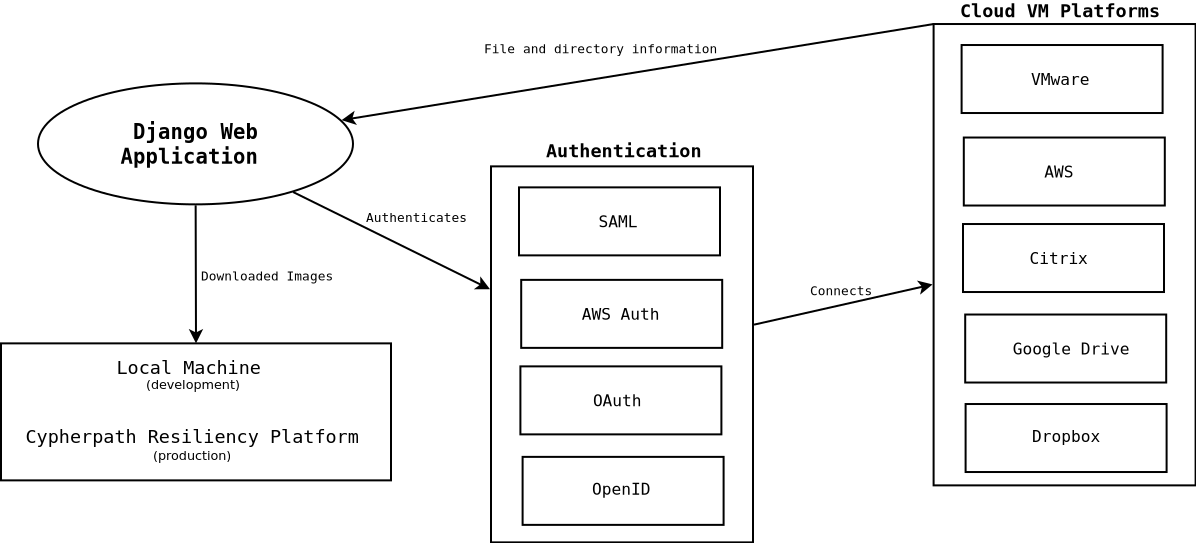
\includegraphics[scale=.4]{downloader_env}
        \caption{A visual representation of the applications environment.}
    \end{figure}


        \subsection{Web Application}
        The software will interact with user as a web application. The web application will prompt the user for things such as
        where their VM services are, and which files to download as well as display information to the user such as what files are available to download.

        The web server that serves the application will be Django's built in development server and when the project is completed, Cypherpath will integrate
        the web application into their existing ecosystem.

        
        \subsection{Authentication API's}
        The application will authenticate to the cloud platforms with various authentication methods and API's. To start with, the application will need to support
        SAML and AWS Authentication, but will need to be designed in a modular fashion so that other authentication methods can be added later on such as OpenID and OAuth.


        \subsection{Cloud Storage API's}
        Once the application is authenticated to a Cloud Storage platform it will gather the directory structure for showing to the user and allowing them to select
        which of their files they would like to download. To start with the application will need to support interacting with VMware and Amazon Web Services. The application will
        need to be designed so that these interactions are modular to enable adding support for other cloud platforms later. Other cloud platforms that will be included, time permitting,
        are Citrix, Google Drive and Dropbox.


        \subsection{Local Storage}
        Once the user has selected which files to download from their cloud platform, the application will download those
        files to the user's local storage. Nothing else needs to be done with the files because after the application is finished
        and Cypherpath has integrated the web application into their platform, they will direct the downloads where they need them.


    \section{Operation}
    In the following sections the operation of the application will be described, including starting the application
    (invocation), the commands the application uses and finally, how to close or terminate the application.

        \subsection{Invocation}
        Since the application will be integrated into Cypherpath's platform, the application will be started using Django's built-in development webserver and
        the user will not need to be authenticated to use the application. To invoke the application the user will simply enter the URL that the application is running on and will
        be presented with the first screen of the application.

        Initially the user will be displayed with an area to enter a URL that their VM's reside at (An AWS or VMware link). If the user has previously entered and logged into one of these
        URL's before then they will also have a list of these to log back into them.

        \subsection{User Actions}
            \subsubsection{Enter URL}
            The user can enter a URL that goes to their cloud platform (VMware or AWS initially). The application will figure out which cloud platform the URL belongs to and then will have the
            user enter their login credentials for that platform. Once authenticated the application will present the user with their files and folders that are on that platform.
            
            \subsubsection{Select URL}
            In addition to the text box to enter a URL the user will also be presented with a list of previously entered URLs. The user will be able to remove URL's from this list, reconnect to them
            or close the session with that cloud platform.

            \subsubsection{Display File Structure}
            Once the user has selected a cloud platform and is authenticated, they will be presented with their directory structure on that platform. From here they can navigate through their folders and
            select multiple files and folders that they wish to download.

            \subsubsection{Download}
            Once the user has selected which files they wish to download and press the download button the application will download those files to the user's local storage. The user won't choose where to store these
            files and where the application stores them won't matter as later on the location will be chosen by Cypherpath.

            \subsubsection{Error Catching}

        \subsection{Termination}
        Since the user is not authenticated to the web application, to terminate their interaction with the application they will simply close the browser tab or window that has the
        application open. The application will keep any authentication tokens for use the next time the user uses the application.


    \section*{References}
    % Reference the project plan?
    % Possibly reference documentation to the various API's?

    \appendix
    \section{Appendix}
    % Sample files, if any?
    % Maybe a sketch of the general page layout?

\end{document}
